\section{Technical Base}

\subsection{Unix-based Operating Systems}

The Unix-based operating systems are a family of operating systems. They all have one thing in common which is that they share the design principle of the original Unix System. Unix was developed in Bell Labs and its predecessor was the Multics system \cite{farrow1991}.  The core characteristics of the Unix system are that it is a general-purpose, interactive and multi-user operating system \footnote{Dennis M. Ritchie and Ken Thompson. The UNIX Time-Sharing System [online] homepage: dsf.berkeley.edu URL: https://dsf.berkeley.edu/cs262/unix.pdf [Accessed 28.11.2025]}.

\subsection{Linux}

\subsubsection{General Aspects}

Linux is an open-source operating system based on Unix. The Linux kernel was created by Linus Torvalds and was first released back in 1991. Linus Torvalds had a kernel but no additional programs like a shell and compilers which together comprise a working system. Richard Stallman and GNU provided the needed programs and together the first version of the Linux operating system was created \footnote{What is Linux. [online] homepage: linux.org URL: https://linux.org/threads/what-is-linux.4106/ [Accessed 28.11.2025]}. Linux is comprised of several different components including the bootloader, kernel, Init system. daemons, graphical server, desktop environment and applications. \footnote{The Linux Foundation. What is Linux? [online] homepage: linux.com URL: https://www.linux.com/what-is-linux/ [Accessed 28.11.2025]}

\subsubsection{Kernel}

The kernel is the core of the operating system. It is the central software which has various critical responsibilities. It first and foremost manages and allocates computer resources like CPU, RAM and devices. It is the connecting tissue between hardware and software and consequently allows users to manage system components like networks, file systems and drivers among other things. \newline\newline The most important tasks performed by the kernel are listed below:

\begin{itemize}
	\item Process scheduling
	\item Memory management
	\item Provision of a file system
	\item Creation and termination of processes
	\item Access to devices
	\item Networking
	\item Provision of a system call application programming interface (API)
\end{itemize}

A very significant concept in this context is the distinction between user mode and kernel mode. Different processes have different rights. A user process should never access kernel addresses. Modern systems including Linux use a split virtual address space. Virtual memory is marked as either being part of user space or kernel space. As a result while CPU is running in user mode it can only access memory which is marked as being in the user space. \newline\newline  Kernel mode is the highest privilege level. There are operations which can only be performed while the CPU is in kernel mode as the operation needs access to memory which is in the kernel space. These operations need access and right to resources a user mode operation should never have. Typical examples of such operations include system call processing and accessing memory-management hardware \cite{kerrisk2010}.

\subsubsection{Daemons}

Daemons are special processes. They are background processes to be more specific, which means they run continuously without direct user interaction as they have no controlling terminal. Many of them are started when the system boots and continues running until the system is shut down\cite{kerrisk2010}.

\subsubsection{Shell}

The shell is also referred to as command interpreter because it captures its functionality. It is a program which acts as an interface between the user and operating system. The user can type in commands which will be executed programs in response to the user's commands. \newline\newline Bash (Bourne again shell) is the commonly used shell on Linux systems. Shells are not just designed for interactive use. Another important feature are shell scripts, which are text files containing shell commands\cite{kerrisk2010}.

\subsubsection{Filesystem}

A filesystem is comprised of serveral components which all put together give it the functionality it needs to do its job\footnote{David Both. An introduction to Linux's EXT4 filesystem. [online] homepage: opensource.com URL: https://opensource.com/article/17/5/introduction-ext4-filesystem [Accessed 29.11.2025]}.

\begin{enumerate}
	\item Data storage: organized collection of files and directories to store and retrieve data
	\item Namespace: methodology which provides rules for naming and organizing data in a hierarchy
	\item Security model: a scheme for defining access rights
	\item API: a set of system calls for navigating and manipulating objects like directories and files
	\item Implementation: software to tie the filesystem components together.
\end{enumerate}

The kernel supports many diverse implementations of filesystems \cite{nemeth2011}. All these filesystems differ in certain aspects of their implementation for example concerning how blocks are allocated or the organization of directories. However programs can not be written in a way to account for all the implementations of filesystems. The virtual file system (VFS) is a kernel feature which provides a solution for this conundrum by creating an abstraction layer for filesystem operations. The concept is a two-way as the VFS defines a generic interface for filesystem operations and in turn each filesystem an implementation of the interface\cite{kerrisk2010}.\newline\newline The default and thereby most common used filesystem on many Linux distributions is ext4 \footnote{Bosko Marijan. Linux File System: Types, Features, Limitations. [online] homepage: phoenixapp.com URL: https://phoenixnap.com/kb/linux-file-system [Accessed 29.11.2025]}.



\setcounter{secnumdepth}{4}
\paragraph{Everything is a file}

 "In Linux everything is a file." is a common phrase. It actually refers to the fact that all system resources like processes, hardware and network connections are represented as files and can be accessed using standard file operations. A file system is commonly divided into data blocks for storing file content and inodes for storing metadata and pointers to the data blocks. Inodes hold the information for any Linux file with the exception of the file's name and data \footnote{Linux basic concepts [online] homepage: microsoft.github.io URL: https://microsoft.github.io/WhatTheHack/020-LinuxFundamentals/Student/resources/concepts.html [Accessed 28.11.2025]}.

\setcounter{secnumdepth}{4}
\paragraph{Single Directory Hierarchy}

It is the responsibility of the kernel to organize all files in the system. In Linux the kernel achieves this by maintaining a single hierarchical directory structure where at its base resides the root directory which is named '/' (slash) \cite{kerrisk2010}. The following picture shows a subset of this single directory hierarchy.

\smallskip
\begin{figure}[h]
\centering
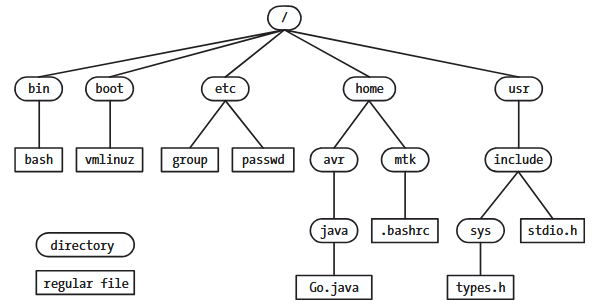
\includegraphics[scale=1, keepaspectratio]{images/single-directory-hierarchy}
\caption{Single Directory Hierarchy \cite{kerrisk2010}}
\end{figure}

\setcounter{secnumdepth}{4}
\paragraph{File Types}

The Linux filesystem has seven file types which are listed below\cite{nemeth2011}:

\begin{itemize}
	\item Regular files
	\item Directories
	\item Character device files
	\item Block device files
	\item Local domain sockets
	\item Named Pipes (FIFOs)
	\item Symbolic links
\end{itemize}

\subsubsection{Distributions}

Linux distributions are also referred as distros and are complete operating systems built on the Linux kernel. A distro includes the kernel, system tools, packet manager bundled with all the other necessary components to be ready for use out of the box. There are hundreds of distros available today, each come with a pre-installed set of programs and each customized to target a different user audience\footnote{Gavin Wright. What is Linux distros (Linux distribution)? [online] homepage: techtarget.com URL: https://www.techtarget.com/searchdatacenter/definition/Linux-distros-Linux-distribution [Accessed 29.11.2025]}.

\subsection{Python}

\subsubsection{General Aspects}

Python is a high-level and interpreted programming language and was created by Guido van Rossum. An interpreter is a program which reads and executes line by line or statement by statement. This contrary to a compiler which translates the entire source code into object code before being executed \cite{downey2012}.  \newline\newline It is a strongly, dynamically typed language. This means that it has a strict type system but variables are in essence simply pointers objects. Objects have a permanent type however variables can point to arbitrary objects.  It is a very versatile language and therefore used in wide array of different fields including web development, automation, data science and artificial intelligence among many others. 

\subsubsection{Scripting Language}

Python is an advanced scripting language which posses high-level data structures. In application scripting the functionality of another program is expanded and is often used in context of automation. Furthermore it is used to interact with the operating system or language binding wrappers in which the code libraries are used to bridge two different languages thereby allowing a library written in one language to be used from another.

\subsubsection{Python and Unix/Linux}

The script to scan Linux machines is written in Python. Below a table of Python libraries used to interact with the Linux operation system in order to find out all the necessary information about the machine to evaluate its status regarding the risks for privilege escalation. \newline

\begin{tabular}{@{} *5l @{}}    \toprule
\emph{Purpose} & \emph{Library}   \\\midrule
Executing Commands & subprocess \\
Filesystem inspection & os, pathlib, shutil \\
Regex parsing & re \\
Process interrogation & os, /proc parsing \\
Serialization & json, pickle, csv\\\bottomrule
 \hline
\end{tabular}

\subsubsection{Command Line Interface}

The goal is to create a more advanced command line interface to facilitate all the required options and ensure a great user experience. The choice for the appropriate library fell on \textit{click}. It offers advanced features such as decorator-based approach to defining commands, automatic argument validation and reusable commands\footnote{Usool. Mastering Command-Line Interfaces (CLI) in Python: A Comprehensive Guide. [online] homepage: dev.to URL: https://dev.to/usooldatascience/mastering-command-line-interfaces-cli-in-python-a-comprehensive-guide-10bc [Accessed 29.11.2025]}. Moreover it capable of handling file handling out of the box and supports implementation of Unix/POSIX command line conventions\footnote{Why Click? [online] homepage: click.palletsproject.com URL: https://click.palletsprojects.com/en/stable/why/ [Accessed 29.11.2025]}.

\subsubsection{BCC - BPF Compiler Collection}

It is a framework for creating eBPF programs which are embedded inside a python a program. The eBPF programs are written in C and BCC features bindings for Python \footnote{BPF Compiler Collection (BCC). [online] homepage: github.com URL: https://github.com/iovisor/bcc [Accessed 30.11.2025]}.


\subsection{Understanding Vulnerabilities}

This section will exam vulnerabilities in context of privilege escalation. We examine the vulnerability and lay out which operating system components are involved, how they are work and why the misconfigurations can lead to the vulnerabilities in the first place. 

\subsection{CVEs API}

The National Institute of Standards and Technology (NIST) provides an API which can be used to retrieve information about CVEs (Common Vulnerabilities and Exposures) from the NVD (National Vulnerability Database)\footnote{NIST. National Vulnerability Database. [online] homepage: nvd.nist.gov URL: https://nvd.nist.gov/developers/vulnerabilities [Accessed 30.11.2025]}. Once a vulnerability is found this service can provide additional information and guidance on how to handle the findings and identifying possible solutions to mitigate the risks. 

\subsection{eBPF}

eBPF stands for extended Berkeley Packet Filter. It is a technology which allows users to run sandboxed programs with privileged access within the Linux kernel without modifying the kernel's source code. Users can write eBPF programs to extend the capabilities of the operating system at run time.  It enables a wide range of applications, including advanced networking, security, and observability \footnote{eBPF Documentation - What is eBPF. [online] homepage ebpf.io URL: https://ebpf.io/what-is-ebpf/ [Accessed 30.11.2025]}. 